\documentclass[aspectratio=43,notes]{beamer}

\usepackage{ngerman}
\usepackage[ngerman]{babel}
\usepackage[T1]{fontenc}
\usepackage[utf8]{inputenc}
\usepackage{aeguill}
\usepackage{minted}

\usetheme{veripeditus}

\title{Veripeditus}
\subtitle{The Free AR Game Framework for Everyone}
\author{Eike Tim Jesinghaus}
\date{\today}
\institute{FOSDEM 2017}

\begin{document}
 \begin{frame}
  \titlepage
 \end{frame}

 \section{About us}


 \begin{frame}
  \frametitle{Eike}

  \begin{itemize}
   \item{Eike Tim Jesinghaus}
   \item{15 year-old student from Germany}
   \item{Python programmer since the age of 11 years}
  \end{itemize}
 \end{frame}

 \note[itemize]{
  \item{Give the audience a feeling of what kind of person you are.}
  \item{Do NOT excuse for this being your first talk, or any other shortcomings you fear.}
 }

 \begin{frame}
  \frametitle{Nik}

  \begin{itemize}
   \item{blablabla}
  \end{itemize}
 \end{frame}

 \section{About Veripeditus}

 \begin{frame}
  \frametitle{What is Veripeditus?}

  \begin{itemize}
   \item{A free software AR game creation framework}
   \item{Allows easy creation of augmented reality games}
   \item{Run your own server with different worlds and different games in them}
   \item{Play the games using any mobile browser}
  \end{itemize}
 \end{frame}

 \note[itemize]{
  \item{Give a short explanation about what Augmented Reality is in the context of Veripeditus.}
  \item{Ask the audience a few questions, like about their experience with AR games, and so on.}
 }

 \begin{frame}
  \frametitle{How it got started}

  \begin{itemize}
   \item{We were looking for a new fun project}
   \item{AR gaming seemed to become popular (cf. that monster catching thingy)}
   \item{We wanted to create something like that without the privacy hassle}
   \item{Many different ideas - why not make it a framework?}
  \end{itemize}
 \end{frame}

 \note[itemize]{
  \item{This is about what we thought when we started the project.}
  \item{Tell a story about how we found Pokémon Go as popular, but non-free, and we wanted our own…}
  \item{Maybe add one or two sentences about privacy being a major issue with popular AR games.}
 }

 \begin{frame}
  \frametitle{New goals after some time}

  \begin{itemize}
   \item{The framework got more and more powerful}
   \item{Developing games with it got much easier than expected}
   \item{So now:
    \begin{itemize}
     \item{Make it as accessible as possible}
     \item{Enable use in various fields besides just-for-fun gaming}
     \item{More about that later!}
    \end{itemize}
   }
  \end{itemize}
 \end{frame}

 \note[itemize]{
  \item{Tell a story about how we tried out a lot of things, had many different ideas.}
  \item{Tell a story about how it got more and more abstract, until we decided to make it a framework.}
  \item{Tell a story about how we got many new ideas, and talked to many people, who had a lot of ideas on how and where Veripeditus could be useful.}
  \item{Tell that we will have a look at the various use fields later.}
 }

 \section{How to create games}

 \begin{frame}
  \Large
  Before we discuss more, let's look at how to make a game!
 \end{frame}

 \note[itemize]{
  \item{This is an interjection so we break lose from just story-telling.}
  \item{The audience should feel that we now show off something.}
 }

 \begin{frame}
  \frametitle{Basic workflow for making a game}

  \begin{enumerate}
   \item{Plan any game objects and their features (position, names, images,…}
   \item{Draft a game plot, activities, other logic}
   \item{Put everything together in object/class definitions in pure Python}
  \end{enumerate}
 \end{frame}

 \note[itemize]{
  \item{Tell a bit about every point.}
  \item{Maybe draft a really simple and quick example for every point, but do NOT give away the example that follows!}
 }

 \begin{frame}
  \frametitle{A first tiny game}

  {
   \inputminted[linenos,breaklines]{python}{ex_schoolkid.py}
  }
 \end{frame}

 \note[itemize]{
  \item{Tell that this is a simple Python module.}
  \item{Ask the audience to read it and think about it a bit.}
  \item{Give 30 seconds or a minute time.}
  \item{Do not explain the code at this point!}
 }

 \begin{frame}
  \Large
  Quiz time: What have we got here?
 \end{frame}

 \note[itemize]{
  \item{Ask the audience to try and explain what the code we showed does.}
  \item{Really motivate them ;)!}
 }

 \begin{frame}
  \frametitle{Quiz time: What have we got here?}

  Answers:

  \begin{itemize}
   \item{A Player object with no special behaviour}
   \item{An NPC (non-player character) named AnyChild
    \begin{itemize}
     \item{Spawning at every building tagged a school on OpenStreetMap}
     \item{Having the image of a schoolkid}
     \item{Saying "I can make AR games :)!" when asked}
    \end{itemize}
   }
  \end{itemize}

  Isn't that cool?
 \end{frame}

 \note[itemize]{
  \item{Congratulate the audience for finding out what the game does so well :)!}
  \item{Repeat all facts, amybe adding or correcting everything that might still be missing.}
 }

 \begin{frame}
  \frametitle{First tiny game, in pictures}

  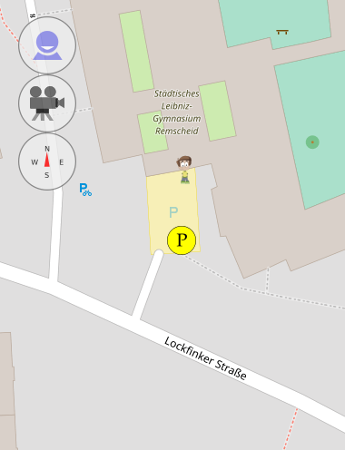
\includegraphics[width=.3\textwidth]{ex_schoolkid_shot1}\hfill
  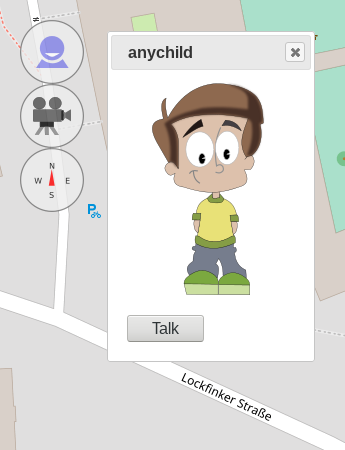
\includegraphics[width=.3\textwidth]{ex_schoolkid_shot2}\hfill
  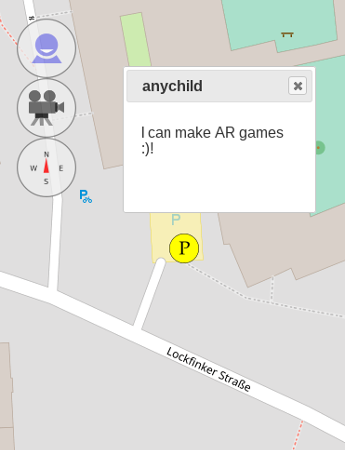
\includegraphics[width=.3\textwidth]{ex_schoolkid_shot3}
 \end{frame}

 \note[itemize]{
  \item{Tell a story about the player walking to the location near the school, seeing the NPC, clicking it and then the talk button, and the NPC sending its response.}
  \item{Add a note that of course, any logic involving conditions, and so on might influence the response in a real game!}
 }

 \section{Framework development and design}

 \begin{frame}
  \frametitle{Framework development and design goals}

  \begin{itemize}
   \item{Make game creation as easy and accessible as possible}
   \item{Still allow adding arbitrarily complex code
    \begin{itemize}
     \item{No DSL - game cartridges are plain and honest Python packages}
     \item{Don't get in the way while still being helpful}
    \end{itemize}
   }
   \item{Provide all basic objects and functions to derive from
    \begin{itemize}
     \item{Player, Items, NPCs, Locations, …}
     \item{Dialogues, item management, inventory management, interaction, …}
    \end{itemize}
   }
   \item{Tight and simple integration with OpenStreetMap}
  \end{itemize}
 \end{frame}

 \note[itemize]{
  \item{Elaborate on the point that the framework offers a lot of abstraction, so using it becomes easy.}
  \item{Elaborate on the point that still, everything is plain Python, and so everything that can be done with Python can be done in a game.}
 }

 \begin{frame}
  \frametitle{Technologies used}

  \begin{itemize}
   \item{Backend
    \begin{itemize}
     \item{Python 3}
     \item{Flask web framework with Flask-Restless, and others}
     \item{SQLAlchemy and OSMAlchemy}
    \end{itemize}
   }
   \item{Frontend
    \begin{itemize}
     \item{HTML 5, JavaScript, CSS 3}
     \item{JQuery and JQuery-UI}
     \item{Leaflet}
    \end{itemize}
   }
   \item{Simple RESTful HTTP API}
  \end{itemize}
 \end{frame}

 \section{State and future}

 \begin{frame}
  \frametitle{What's already there}

  \begin{itemize}
   \item{Framework features and objects
    \begin{itemize}
     \item{Items and NPCs}
     \item{Spawning at lat/lon or OSM objects}
     \item{Interaction (collecting items and talking to NPCs}
    \end{itemize}
   }
   \item{Backend technology with advanced API}
   \item{Reference web application for gameplay
    \begin{itemize}
     \item{Map view}
     \item{Camera / 3D view}
    \end{itemize}
   }
   \item{Advanced debugging/testing mode for easier development}
  \end{itemize}
 \end{frame}

 \note[itemize]{
  \item{Tell a bit about what you can do with every of the aspects.}
 }

 \begin{frame}
  \frametitle{Many different use fields}

  \begin{itemize}
   \item{Gaming, of course…
    \begin{itemize}
     \item{Create just-for-fun outdoor games with AR aspects}
    \end{itemize}
   }
   \item{Educational use
    \begin{itemize}
     \item{Coding lessons
      \begin{itemize}
       \item{Basic coding}
       \item{Object-oriented modelling}
       \item{Databases, APIs, and much more}
      \end{itemize}
     }
     \item{Interdisciplinary use
      \begin{itemize}
       \item{Educational games for history, arts, …}
       \item{Fun at field trips}
      \end{itemize}
     }
    \end{itemize}
   }
   \item{Tourism and attractions
    \begin{itemize}
     \item{Interactive stories in open air museums, …}
    \end{itemize}
   }
  \end{itemize}
 \end{frame}

 \note[itemize]{
  \item{Give an explanation and a short example about every of the aspects.}
  \item{Elaborate on how Veripeditus can improve computer classes, by combining gaming interests of the students with Python in a framework that can be used at all experience levels.}
  \item{Elaborate on how AR games could be used in other subjects.}
 }

 \begin{frame}
  \Large
  Spontaneous question: Any quick ideas here?
 \end{frame}

 \note[itemize]{
  \item{Motivate the audience to name any ideas they might have right now.}
 }

 \begin{frame}
  \frametitle{Coming up / Roadmap}

  \begin{itemize}
   \item{Improvements to web application}
   \item{Interactive / live game code editor}
   \item{More detailed and diverse game object interactions}
   \item{WebGL 3D models}
   \item{Sound support}
   \item{HUD defined by games}
   \item{3D interaction with game objects (aiming, etc.)}
   \item{…}
  \end{itemize}
 \end{frame}

 \note[itemize]{
  \item{Report that Veripeditus is only one year old and we first want to make basic things work very well.}
  \item{Elanorate a bit on the list of ideas that are already on the roadmap.}
 }

 \section{You and us and Veripeditus}

 \begin{frame}
  \frametitle{What we can do for you}

  \begin{itemize}
   \item{Make Veripeditus a framework for YOU to use}
   \item{Help you implement game ideas in your use fields}
  \end{itemize}
 \end{frame}

 \note[itemize]{
  \item{Elaborate on how we really want to make Veripeditus a good tool for everyone who has a use for AR gaming.}
  \item{Elaborate on how we will be very happy to see all new thoughts and help out with doing some cool things with Veripeditus.}
 }

 \begin{frame}
  \frametitle{What you can do for us to help us help you}

  \begin{itemize}
   \item{Report your ideas, feature requests and bugs}
   \item{Help us if you are (or want to be) a JavaScript or CSS guru}
   \item{Test Veripeditus on many mobile devices}
   \item{Tell us stories from active usage in different fields}
  \end{itemize}
 \end{frame}

 \note[itemize]{
  \item{Tell the audience that we have many ideas, but are unexperienced with some topics.}
  \item{Ask specifically for help withthe web application, concerning JavaScript and CSS 3 3D transformations.}
 }

 \begin{frame}
  \frametitle{Where to find us}

  \begin{itemize}
   \item{GitHub: \url{https://github.com/Veripeditus/veripeditus-server}
    \begin{itemize}
     \item{Please find up-to-date contact and testing information there!}
     \item{Go mad reporting ideas, questions, requests and bugs}
    \end{itemize}
   }
   \item{Twitter: \href{https://www.twitter.com/VeripeditusTeam}{@VeripeditusTeam}
    \begin{itemize}
     \item{Please follow us to receive updates!}
    \end{itemize}
   }
   \item{E-mail: \href{mailto:team@veripeditus.org}{\nolinkurl{team@veripeditus.org}} }
  \end{itemize}
 \end{frame}

 \note[itemize]{
  \item{Tell the audience that there will be news on the upcoming release within the near future.}
  \item{Motivate the audience to follow us on Twitter and/or GitHub right now.}
 }
\end{document}
